\documentclass{standalone}
\usepackage{tikz}

\usetikzlibrary{calc}


\begin{document}

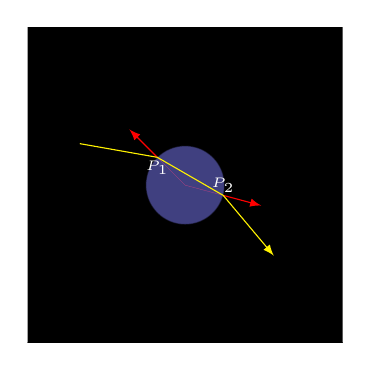
\begin{tikzpicture}
  \path[clip] (-2,0) rectangle (2,4);
  \draw[fill=black,black] (-3,0) rectangle (3,4);


  \coordinate (center) at (0,2);
  \coordinate (entry) at ($ (center) + (135:0.5) $);
  \coordinate (exit) at ($ (center) + (-15:0.5) $);

  \draw[thin,red,ultra thin] ($ (entry) + (135:0) $) -- ($ (entry) + (135:-0.5) $);
  \draw[thin,red,-latex] (entry) -- ($ (entry) + (135:0.5) $);
  \draw[thin,red,ultra thin] ($ (exit) + (-15:0) $) -- ($ (exit) + (-15:-0.5) $);
  \draw[thin,red,-latex] (exit) -- ($ (exit) + (-15:0.5) $);
  \draw[fill=blue!50,opacity=0.5] (0,2) circle [radius=0.5cm];
  \draw[yellow,-latex] ($ (entry) + (170:1) $) -- (entry) -- (exit) -- ++(-50:1);

  \node[white,font=\tiny,below,inner sep=1pt] at (entry) {$P_1$};
  \node[white,font=\tiny,above,inner sep=1pt] at (exit) {$P_2$};
\end{tikzpicture}

\end{document}